\documentclass[a4paper,12pt]{thesis-ekf}
\usepackage[T1]{fontenc}
\usepackage{pdfpages}
\PassOptionsToPackage{defaults=hu-min}{magyar.ldf}
\usepackage{fancyvrb,listingsutf8,xcolor,caption}
\usepackage{fancyhdr,amsthm,amsmath,amssymb,listings}
\usepackage{hyperref}
 \usepackage[T1]{fontenc}
\usepackage[magyar]{babel}
\definecolor{dkgreen}{rgb}{0,.6,0}
\definecolor{dkblue}{rgb}{0,0,.6}
\definecolor{dkyellow}{cmyk}{0,0,.8,.3}
\lstset{
	inputencoding=utf8/latin2,
	language=php,
	basicstyle=\footnotesize\ttfamily,
	numbers=left,
	firstnumber=1,
	breaklines,
	postbreak=\hbox{$\color{red}\hookrightarrow\ $},
	xleftmargin=2cm,
	xrightmargin=2cm,
	backgroundcolor=\color{gray!10},
	frame=tlbr,
	framesep=3pt,
	keywordstyle=\bfseries\color{blue},
	commentstyle=\itshape\color{teal},
	stringstyle= \color{red},
	identifierstyle=\color{dkgreen},
	emph=[1]{php},
	emphstyle=[1]\color{black},
	emph=[2]{if,and,or,else},
	emphstyle=[2]\color{dkyellow},
	showstringspaces=false,
	extendedchars=true,
	literate={á}{{\'a}}1 {é}{{\'e}}1 {í}{{\'i}}1 {ó}{{\'o}}1 {ö}{{\"o}}1 {ő}{{\H{o}}}1 {ú}{{\'u}}1 {ü}{{\"u}}1 {ű}{{\H{u}}}1,
	keywords ={\_\_halt\_compiler, abstract, and, array,
		as, break, callable, case, catch, class,
		clone, const, continue, declare, default,
		die, do, echo, else, elseif,
		empty, enddeclare, endfor, endforeach, endif,
		endswitch, endwhile, eval, exit, extends,
		final, finally, for, foreach, function,
		global, goto, if, implements, include,
		include\_once, instanceof, insteadof,
		interface, isset, list, namespace,
		new, or, print, private, protected, public,
		require, require\_once, return, static,
		switch, throw, trait, try, unset, use, var,
		while, xor, yield,
	}
}
\theoremstyle{definition}
\newtheorem{definicio}{Definíció}[chapter]
\DeclareMathOperator{\tg}{tg}
\setlength{\headheight}{15pt}
\renewcommand{\lstlistingname}{k\'od}

\begin{document}
	\institute{Matematikai és Informatikai Intézet}
	\title{Webservice Menedzselhető Beléptetőrendszerhez}
	\author{Dombi Tibor Dávid\\Programtervező Informatikus Bsc.}
	\supervisor{Dr. Tajti Tibor\\Egyetemi Adjunktus}
	\city{Eger}
	\date{2022}
	\maketitle
	\tableofcontents
	
	\chapter*{Bevezetés}\label{ch-ThesisIntro}
	Már egyetemi tanulmányaim előtt is legjobban a webes alkalmazások készítése foglalkoztatott, és ez az irány megmaradt végig a tanulmányaim során. Nem meglepő, hogy szakdolgozatomnak is ilyen témát választottam.
	Az utolsó két évemben elkezdtem komolyabban foglalkozni az IoT eszközökkel, és mivel rendkívül érdekesnek találtam a témát, szerettem volna belevenni a szakdolgozatomba.
	
	Így született meg ez a dolgozati téma: Egy menedzselhető, online felületen elérhető beléptetőrendszer prototípusa. A feladat rendkívül aktuális, hiszen a legtöbb cég szabályozza, hogy ki léphet be a telephelyére, illetve valamilyen módon naplózza, hogy dolgozói mikor érkeztek és távoztak. Ez a rendszer mindkét feladatot automatizálja.
	
	A projekt elkészítése alatt nagy hangsúlyt fektettem a költséghatékonyságra illetve arra, hogy minél felhasználóbarátabb legyen, mindezt úgy, hogy minden szükséges szolgáltatást megvalósítson.
	
	A piacon számtalan hasonló rendszert találni, de ezek mind rendkívül komplexek és költségesek, többnyire csak a szolgáltató szerelői tudják beszerelni és üzemben tartani, valamint alig-, vagy egyáltalán nem szabhatók személyre. A célom az volt, hogy a projekt megoldást kínáljon ezekre a problémákra. Itt megjegyezném, hogy a dolgozat csak a webservice-al foglalkozik, a hardveres feladatokkal nem, viszont biztosít egy általános interfészt, amihez bármilyen hardver komponenst csatolhatunk.
	
	A technológia kiválasztásánál az volt a célom, hogy minél általánosabb, és minél könnyebben hozzáférhető legyen. Az online elérés megvalósítására számtalan módszer van, de a legegyszerűbb, ha eleve az egész rendszer egy szerveren fut, és valamilyen webtechnológiával van megvalósítva. Ez magában hordozza azt az előnyt is, hogy így a program bármilyen platformról elérhető. Bár a PHP népszerűsége sokat zuhant az elmúlt években\cite{octoverse}, még mindig az egyik legdominánsabb nyelv, ha szerver oldali programozásról van szó\cite{phpstatistics}, így erre esett a választásom. Továbbá, a Node.js vagy Go lang alapú technológiákhoz képest jóval egyszerűbb olcsó, vagy kisebb adatforgalom esetén akár ingyenes tárhely szolgáltatót találni.
	
	\chapter{Rendszer Bemutatása}\label{ch-SystemIntro}
		A rendszer rendkívül moduláris, így könnyen személyre szabható. De általánosítva, csupán egy webservice-ként üzemel, amihez Rest API-on keresztül csatlakozhatunk. Fontos megjegyezni, hogy a projekt nem arra szolgál, hogy programozási tudás nélkül beüzemelhető legyen, de nem is arra, hogy szolgáltatásként nyújtsuk. A projekt célja, hogy egy részletes, átfogó alapot adjon azoknak a fejlesztőknek, akik szeretnék a saját rendszerüket kifejleszteni.
		
		\section{Példa üzem}
		Legyen adott egy vállalkozás, ami szeretné a székhelyéül szolgáló iroda épületet biztosítani, továbbá nyomonkövetni, hogy a dolgozók mikor érkeznek és mikor távoznak az épületből. A cég eleve mikrokontrollerekkel foglalkozik, így a hardware-es kiépítés nem jelent problémát. Ebben az esetben nyúlhatnak olyan projektekhez, mint a jelen szakdolgozati munka.
		
		\emph{\nameref{sc-Installation}} után a program egy egyszerű Rest API szolgáltatás. A kommunikáció JSON formátumban történik. 
		
		A hardware-es megvalósításra javaslat a \ref{ch-Hardware}. fejezetben található. Megvalósítástól függetlenül, a zárnak el kell küldenie a Webservice-nek a saját azonosítóját, illetve a dolgozó azonosítóját (ez lehet például az a szám amit egy RFID kártyáról leolvasott). A zárnak azonosítania kell magát. Ennek mikéntjét az \emph{\nameref{sc-auth} (\ref{sc-auth})} fejezetben részlet\-ezem. A webservice az ismert szabályok alapján eldönti, hogy az adott dolgozó ebben az időpontban használhatja-e a zárat, majd a döntésével válaszol a zárnak. A döntés naplózásra kerül.
		
		Az adminisztrátori felületen követhetjük, mind a rendszerben történt eseményeket, mind a zárak használatát.
		
		\section{Telepítés}\label{sc-Installation}
		 A projekt letölthető a saját github repository-jából\cite{repo}. Az alkalmazás futtatásához szükségünk lesz egy PHP szerverre (nginx, Apache, lighttpd, stb.)\cite{php-servers}, illetve egy Laravel által támogatott adatbázis szerverre (MariaDB, MySQL, Postgres, SQLite, vagy SQL Server)\cite{supported-dbms}. Ezek lehetnek a felhőben, vagy egy lokális szerveren. 
		
		A példa vállalkozásunk kétféleképpen használhatja a programot. Felállíthatják maguk a szükséges rendszert, vagy \verb|Docker| használatával előre beállított \verb|container|-eket is használhatnak, köszönhetően a Laravel Sail támogatásnak\cite{sail-intro}. Bár utóbbit telepíteni jóval gyorsabb, és szinte egyáltalán nem kell belenyúlnunk, saját teszteléseim alapján jelentős teljesítmény csökkenést jelent. Azt, hogy melyik módszert szeretné használni a vállalkozás, kiválaszthatja a \nameref{ssc-install-wizard}ban.
		
		\subsection{Rendszerigény és környezeti követelmények}
		Ahhoz hogy az alkalmazást el tudjuk indítani biztosítanunk kell bizonyos előkövetelményeket. Ezekből két csoportot gyűjöttem össze, attól függően, hogy \verb|Docker|-el szeretnénk-e használni vagy sem.
		
		Amire mindenképpen szükség van:
		\begin{itemize}
          \item \verb|Internet elérés| (a package-ek telepítéséhez)
          \item \verb|Node.js 14.x| vagy újabb (az alapvető segéd script-ek futtatásához)
          \item \verb|Yarn 1.x.x|
        \end{itemize}
        
        Amennyiben \verb|Docker|-el szeretnénk futtatni, úgy csak magát a Docker-t kell feltelepítenünk a fentebbiek mellett. Ellenkező esetben a következőkre van még szükségünk:
        
        \begin{itemize}
            \item \verb|Web szerver| (\verb|Apache|, \verb|NGINX|, stb.)
            \item \verb|PHP 8.1|
            \item \verb|Composer 2.x|
            \item \verb|Laravel kompatibilis DBMS| (\verb|MySQL|, \verb|SQLite|, \verb|MS SQL Server|, \verb|Oracle SQL|)\cite{supported-dbms}
            \item \verb|Redis server| (Cache-eléshez, opcionális)
            \item \verb|NG CLI| (Frontend-hez)
            \item \verb|Ionic CLI| (Frontend-hez)
        \end{itemize}
		
		\subsection{Telepítő varázsló}\label{ssc-install-wizard}
		A telepítő varázsló forráskódja a \verb|scripts/install-wizard.js| fájlban található\cite{install-wizard-js}. Miután a projekt gyökérkönyvtárában feltelepítjük a package-eket (\verb|yarn| parancs\cite{yarn}) automatikusan elindul ez a fájl (\verb|postinstall|). A script végig vezet bennünket a projekt konfigurációján. Ennek egy részletét látni a \ref{fig-install-wizard} ábrán.
		
		\begin{figure}[ht]
        	\centering
        	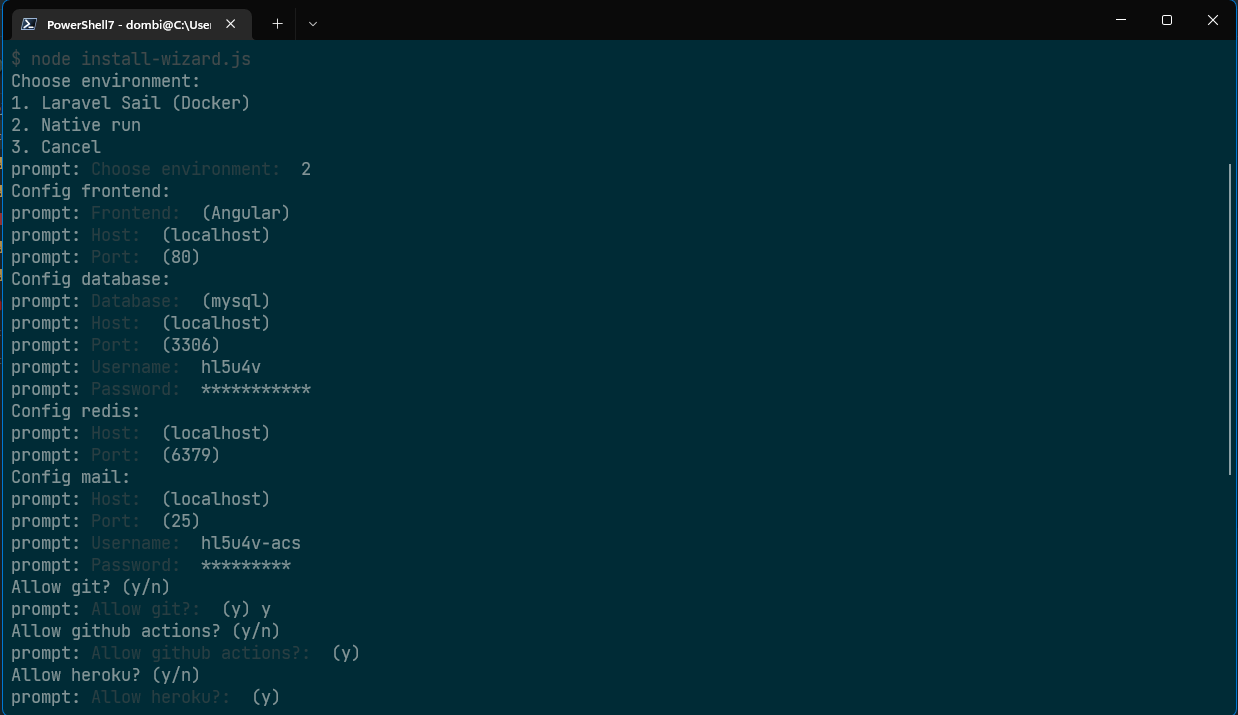
\includegraphics[width=1\textwidth]{images/install-wizard.png}
        	\caption{A telep\'it\H{o} var\'azsl\'o fel\"ulete}
        	\label{fig-install-wizard}
        \end{figure}
		
		Elsőként azt kell kiválasztanunk, hogy \verb|Docker|-ben vagy anélkül (\verb|native run|) szeretnénk futtatni az alkalmazást. Választásunktól függetlenül a következő lépés az alkalmazás elérési címének, és portjának beállítasa, majd pedig az adatbázis kapcsolat beállítása lesz. A telepítő végén opcionálisan egyéb szolgáltatásokat is konfigurálhatunk, úgy mint \verb|Redis| cache, \verb|Mail service|\cite{laravel-mail}, \verb|Git|, illetve CI/CD \verb|Github actions|\cite{gh-actions}-el és \verb|Heroku|-val.
		
		Amennyiben a Docker-t választottuk további feladatunk nincs, elegendő elindítani a \verb|container|-jeinket\footnote{Releváns dokumentáció: https://docs.docker.com/compose/reference/up/} és az alkalmazás készen áll, hogy felvigyük a megfelelő erőforrásokat (lásd \ref{sc-resources} fejezet).
		
		\subsection{Tesztelés és CI/CD}\label{ssc-CiCd}	
		A projekt tartalmazza a PHP Unit csomagot, amivel, nevével ellentétben nem csak unit teszteket fogunk tudni írni, hanem Feature, Database és egyéb teszteket is. Tesztjeink többsége unit tesztnél magasabb szintű teszt lesz, így ezeket fejtem ki bővebben.
		
		Feature teszt írásához örököltessük a teszt osztályunkat a \verb|HttpTest| absztrakt osztálytól. Ekkor elérjük a Laravel beépített Http test funkcióit, illetve további segéd fügvényeket. Ezeknek előnye, hogy a \textqq{beszédes} függvényekkel a tesztünk könnyen olvasható lesz.
		
\begin{lstlisting}[caption={Feature teszt p\'elda},captionpos=b]
<?php

namespace Tests\Feature;

use Tests\HttpTest;
use Utils\StatusCodes;

class ExampleTest extends HttpTest
{

  public function testApiRequest()
  {
    $response = $this->actingAs(Admin())
                     ->postJson(
                       '/api/user',
                       ['name' => 'John']
                     );

    $response->assertStatus(StatusCodes::CREATED)
             ->assertJson(['created' => true]);
  }
  
}
\end{lstlisting}

		A Console Test lényegében Feature teszt, ami a saját Artisan parancsainkat hivatott ellenőrizni. Erre nem írtam külön segéd osztályt, a teszt osztályunkat örököltessük a \verb|TestCase| osztálytól (Ez a Laravel beépített teszt facade osztálya). Kiemelnék egy példát a \href{https://laravel.com/docs/9.x/console-tests#input-output-expectations}{Laravel dokumentációból}\cite{artisan-test}:
		
\begin{lstlisting}[caption={Egy p\'elda Artisan parancs},captionpos=b]
/** Az Artisan parancs: **/
Artisan::command('question', function () {
  $name = $this->ask('What is your name?');

  $language = $this->choice('Which language do you prefer?', [
    'PHP',
    'Ruby',
    'Python',
  ]);

  $this->line('Your name is '.$name.' and you prefer '.$language.'.');
});
\end{lstlisting}

\begin{lstlisting}[caption={A fenti parancs tesztel\'ese},captionpos=b]
/** Test a console command. **/
public function test_console_command()
{
  $this->artisan('question')
       ->expectsQuestion('What is your name?', 'Taylor Otwell')
       ->expectsQuestion('Which language do you prefer?', 'PHP')
       ->expectsOutput('Your name is Taylor Otwell and you prefer PHP.')
       ->doesntExpectOutput('Your name is Taylor Otwell and you prefer Ruby.')
       ->assertExitCode(0);
}
\end{lstlisting}

		Végül pedig az adatbázis tesztekhez elérhető egy \verb|DatabaseTest| absztrakt osztály, melynek célja és használata is hasonló, mint az \verb|HttpTest| osztálynak, csupán más függvényeket tesz elérhetővé. Kiemelném, hogy mind az \verb|HttpTest| mind a \verb|DatabaseTest| a Laravel beépített \verb|TestCase| osztályától örököl, tehát a keretrendszer beépített függvényei mindenkor rendelkezésünkre állnak.
		
		Azért, hogy a felhasználó minél hamarabb megkapja a programját, illetve, hogy a hibák minél hamarabb kiderüljenek és minél hamarabb orvosolhatók legyenek, a modern programozási feladatok legnagyobb része használ valamilyen Continuous Integration-t és Continuous Deployment-et biztosító szolgáltatást (\texttt{CI/CD}). Amennyiben nagyobb mértékben szeretnénk tovább fejleszteni a projektet, mindenképpen érdemes elgondolkodnunk ezek használatán.\cite{ci-cd}
		
		A projekt majdnem teljesen konfigurálva érkezik Github actions (CI) illetve Heroku (CD) számára, így elég a projekt specifikus adatokat megadni (felhasználó nevek, API kulcsok, stb.), és már is használhatóak ezek a technológiák is. Hogy pontosan mit kell beállítanunk, az attól függ, hogy milyen szolgáltatást veszünk igénybe, de a környezeti változókat minden esetben fel kell vinnünk (adatbázis hozzáférés, levelező szerver hozzáférés, stb.).
		
	\chapter{API kommunikáció}
		A webservice egy RESTful API-t biztosít, hogy a saját eszközeink könnyedén tudjanak kommunikálni vele. Az erőforrásaink ebben az esetben a \emph{zárak}, \emph{dolgozók}, \emph{ezek csoportjai}, valamint a \emph{szabályok}. Ezekre a BREAD műveleteket (\ref{sc-bread}) (Browse, Read, Edit, Add, Delete) úgy tudjuk alkalmazni, hogy az API megfelelő végpontjait érjük el, megfelelő HTTP metódussal (GET, POST, PUT/PATCH, DELETE).\cite{rest-api}
		
		Az összes végpont, és azok válaszainak a leírását egy OpenAPI definíciós fájlban megadtam, és a  \href{https://github.com/dombidav/hl5u4v-thesis/blob/main/docs/openapi.json}{szakdolgozathoz csatoltam}\cite{open-api}, így ezeket itt nem fejtem ki, továbbá megtekinthető \href{https://hl5u4v-thesis.stoplight.io/docs/hl5u4v-thesis/branches/main/}{online} is a Stoplight.io felületén is\cite{stoplight}.
		
		\section{BREAD vagy CRUD műveletek}\label{sc-bread}
			Az erőforrásokkal végezhető műveletekről beszélve gyakran használjuk a CRUD vagy BREAD mozaikszavakat. A CRUD a \emph{Create, Read, Update, Delete} szavak rövidítése. Gyakran használják mivel közvetlenül megfeleltethető mind az SQL nyelv metódusainak, mind az HTTP metódusainak, ezt látjuk a \ref{table:http-sql-crud} táblázaton.
			
			\begin{table}[h!]
				\centering
				\begin{tabular}{|c | c | c|}
					\hline
					\multicolumn{1}{|c|}{\textbf{SQL}} & \textbf{CRUD} & \textbf{HTTP} \\ \hline
					INSERT & CREATE & POST \\ \hline
					SELECT & READ & GET \\ \hline
					UPDATE & UPDATE & PUT / PATCH \\ \hline
					DELETE & DELETE & DELETE \\ \hline
				\end{tabular}
				\caption{HTTP, SQL, és CRUD műveletek megfeleltetése}
				\label{table:http-sql-crud}
			\end{table}
		
			Egy másik megközelítés, a BREAD (Browse, Read, Edit, Add, Delete). Ez lényegében megegyezik a CRUD metódusokkal, annyi különbséggel, hogy a BREAD külön veszi azt a metódust, amikor minden erőforrásra kíváncsiak vagyunk (Indexelés), illetve azt a metódust amikor csak egy erőforrás részleteire vagyunk kíváncsiak. Ez azért előnyösebb a számomra, mert ezek jobban megfeleltethetők a Laravel Controller metódusainak. Ha ezeket is meg szeretnénk feletetni egymással, akkor a táblázatunk módosul\cite{bread}, ez látszik a \ref{table:http-sql-crud-bread} táblázaton.
 	
			\begin{table}[h!]
				\centering
				\begin{tabular}{|c|c|c|c|c|}
					\hline
					\textbf{SQL} & \textbf{CRUD} & \textbf{HTTP} & \textbf{BREAD} &\textbf{Laravel Controller} \\ \hline
					SELECT & READ & GET & BROWSE & INDEX \\ \hline
					SELECT & READ & GET & READ & SHOW \\ \hline
					UPDATE & UPDATE & PUT / PATCH & EDIT & UPDATE \\ \hline
					INSERT & CREATE & POST & ADD & STORE \\ \hline
					DELETE & DELETE & DELETE & DELETE & DESTROY \\ \hline
				\end{tabular}
				\caption{HTTP, SQL, CRUD műveletek a BREAD-hez képest}
				\label{table:http-sql-crud-bread}
			\end{table}	
		
		\section{HTTP metódusok}
			Az HTTP szabvány úgynevezett metódusokat (\emph{methods}) definiál nekünk\cite{http}, hogy ezzel közöljük a szerverrel, hogy mi a szándékunk az URI-ben megnevezett erőforrással.\cite{uri} Vegyük példáúl a \verb|worker| erőforrást. Ebben az esetben az implementált metódusok a következők:
			
			\subsection{GET}
				Ezen HTTP metódussal két funkció is elérhető. Ha nem definiáljuk hogy pontosan melyik rekordot (példákban: melyik dolgozót) szeretnénk részletezni egy erőforráson belül, akkor vissza kapjuk az összes ezen erőforrásban tárolt rekordot (tehát az összes dolgozót). A Laravelben megegyezés szerint ez a függvény az \verb|index()|.
\begin{lstlisting}[caption={P\'elda a BROWSE met\'odusra},captionpos=b][language=json]

Request:
 GET www.example.com/worker
 
Response body:
 [
   {
     "name": "Shelia Lakin",
     "created_at": "2021-06-30T12:09:20.478Z",
     "phone": "938-402-3157 x810",
     "id": "4b3403665fea6"
   },
   {
     "name": "Whitney McClure",
     "created_at": "2021-06-18T05:26:38.641Z",
     "phone": "(765) 538-9079",
     "id": "4b3407665bcd5"
   }
]
\end{lstlisting}
				
				Amennyiben az URI-ben specifikáljuk, hogy melyik rekordot szeretnénk elérni, úgy részletes információkat kapunk arról (tehát egy dolgozó adatait kapjuk vissza). Laravelben ez a \verb|show()| függvény, konvenció szerint.
\begin{lstlisting}[caption={P\'elda a READ met\'odusra},captionpos=b][language=json]

Request:
 GET www.example.com/worker/4b3403665fea6
 
Response body:
 {
   "name": "Whitney McClure",
   "created_at": "2021-06-18T05:26:38.641Z",
   "last_logged_in": "2021-06-30T05:26:38.641Z",
   "phone": "(765) 538-9079",
   "id": "4b3407665bcd5",
   "teams": [
     {
       "id": 1,
       "name": "Team1"
     },
     {
       "id": 2,
       "name": "Team2"
     }
   ]
 }
\end{lstlisting}

			\subsection{POST}
				Ezzel a metódussal új erőforrást hozhatunk létre. Ehhez a kérésünk törzsében meg kell adnunk minden szükséges tulajdonságot, illetve az opcionális tulajdonságokat vagy megadjuk, vagy nem. Ezen tulajdonságok sorrendje tetszőleges. A kérésünk törzsében lehet egy JSON objektum vagy egy tömb, ami több objektumot is tartalmazhat. Ha ez utóbbi áll fent, akkor a webservice felveszi nekünk az összes rekordot. Ez a felvétel tranzakció szerűen működik, tehát ha bármelyik adatfelvitel sikertelen, akkor az összes visszavonásra kerül. Ha az adatfelvitel sikeres a szerver 201-es státuszkóddal válaszol. Ez a Laravel-ben a \verb|store()| függvény.
				
			\subsection{PUT és PATCH}
				Ez a két metódus nagyon hasonló egymáshoz, azonban van két nagyon fontos különbség: A PUT metódust használva az általunk megadott adatok \emph{felülírják} azt a rekordot, amit az URI-ben azonosítottunk. Ez azt jelenti, hogy ha részleges adatot küldünk, akkor csak ezek tárolódnak le, minden más elveszik. A PATCH ehhez képest kifejezetten részleges adatot vár, és csak a kapott tulajdonságokat módosítja. 
				
				A másik különbség abban van, hogy hogyan kezelik azt az esetet, amikor nem létezik a rekord, amit el szeretnénk érni: A PUT ilyenkor egyszerűen létrehozza azt, a PATCH viszont hibát ad 404-es státuszkóddal.
				
				A Laravel alap beállításai alapján nem tesz különbséget a PUT és a PATCH között, de ezt megváltoztathatjuk. Mivel gyakorlatban többnyire csak a PATCH metódus lesz használva, csak ezt implementáltam, és megtartottam a Laravel alap beállítását. Tehát mind a két metódus az \verb|update()| függvényt éri el.
				
			\subsection{DELETE}
				Laravelben ez a \verb|destory()| függvény. A metódus neve elárulja a funkcióját is. Ezt a végpontot elérve, a webservice eltávolítja a URI-ben azonosított rekordot, majd a válaszban visszaküldi a kliensnek az eltávolított rekord részleteit, mint a \verb|show()| függvény, azonban ez a rekord már nem szerepel az adatbázisban.
		
		\section{Azonosítás}\label{sc-auth}
			Mint minden webszolgáltatásnál itt is szükséges szabályozni a hozzáférést. Erre a Laravel Sanctum\footnote{Forráskód: \url{https://github.com/laravel/sanctum}} csomagot kombináltam a \verb|php-open-source-saver/jwt-auth| csomaggal\footnote{Forráskód: \url{https://github.com/PHP-Open-Source-Saver/jwt-auth}}. Utóbbi csomag az egyik legkedveltebb, és legrobosztusabb JWT csomag ami csak elérhető PHP-hoz. A Sanctum-ra azért van szükség, mert így a hitelesítést el lehet végezni a Laravel beépített Policy rendszerén keresztül\cite{sanctum}. A JWT token elküldhető fejlécben, sütiként, vagy akár az üzenet törzsében is.
			
			\subsection{JWT}
			A JWT (JSON Web Token) egy szabvány (\href{https://tools.ietf.org/html/rfc7519}{RFC 7519}), aminek a célja, hogy biztonságosan lehessen üzeneteket küldeni egyszerű JSON objektumokként. Az üzenet minden esetben digitálisan alá is van írva. Bár az üzenet lehet titkosított is, ebben az alkalmazásban csak az aláírást használtam.\cite{jwt-intro}
			
			A JWT kompakt formája három darab Base64-URL kódolt szöveg. \cite{jwt-intro}
			
			Az első rész a fejléc, egy JSON objektum, aminek két mezője van. Az első az üzenet típusa (\emph{typ}). Ennek az értéke mindig \emph{JWT}. A második az algoritmus (\emph{alg}), amit az aláíráshoz használtunk (\emph{HMAC}, \emph{SHA256} vagy \emph{RSA}, utóbbi esetén publikus-privát kulcs generálandó, így a kliens is meggyőződhet róla, hogy a szerver küldte az üzenetet, és nem egy harmadik fél).\cite{jwt-handbook} 
			
			Ebben a projektben az \emph{HMAC} algoritmust használtam, mivel a projekt volumenéhez mérten elegendőnek találtam.
			
			A második rész a \emph{payload}. Ide adhatunk hozzá minden olyan mezőt, amire a kliensnek szüksége van. Bár semmi sem akadályoz minket abban, hogy kedvünkre bármilyen kulcsot (\emph{claim}) hozzáadjunk, vannak bizonyos mezők, amiknek a neveit és tartalmukat szabvány írja elő. Ezek megtekinthetők az \href{https://datatracker.ietf.org/doc/html/rfc7519#section-4.1}{IETF} által nyilvántartott RFC-ben (\emph{Registered Claims}, ezek a JWT szabvány részei), illetve a \href{https://www.iana.org/assignments/jwt/jwt.xhtml}{IANA nyilvántartásában} is (\verb|Public Claims|, ezek regisztrációját kérték). 
			Minden más \emph{claim} úgy nevezett \emph{Private Claim}.\cite{jwt-intro}
			
			Ebben a projektben ilyen \emph{Private Claim} a \emph{user}, amiben az aktuális user alapvető adatai vannak. Ezek az adatok használhatók frontend-en történő megjelenítésre, illetve, amikor egy későbbi kérésnél a kliens elküldi ezt a token-t, a webservice-nek nem kell kikeresnie a felhasználót az adatbázisból. Mivel a token-ek nem titkosítottak privát jellegű információt nem csomagolok ebbe az üzenetbe.
			
			A JWT utolsó része egy digitális aláírás. Az aláírást a webservice végzi, egy szerveren tárolt 32 bájt hosszú titkos kulcs segítségével. Mivel a kulcs titokban van tartva, így a webservice bejövő üzenetnél ellenőrizheti, hogy módosították-e a \emph{payload} tartalmát. Amennyiben az üzenet módosult, a webservice eldobja azt.
			(Amennyiben \emph{RSA} algoritmust használtunk a kliens ezt az alírást ellenőrizheti.)\cite{jwt-handbook}
			
			\subsection{Bejelentkezés}
    			A felhasználó bejelentkeztetése úgy történik, hogy a felhasználó egy \emph{POST} kérést indít az \verb|api/auth/signin| végpontra. Az üzenet tartalma (\verb|Request body|) az email címe és a jelszava. A backend ezt validálja. Amennyiben ez a validáció sikeres, úgy a backend az azonosított felhasználó adatait a válasz JWT \verb|payload| részébe csomagolja, \verb|private claim|-ként, majd az egészet egy titkos kulcs alapján aláírja.\cite{jwt-workflow} Az aláíráshoz használt algoritmus \emph{HS256}. 
    			Itt kiemelném, hogy ez a token nincs titkosítva, csak alírva.
    			
    			Amikor a felhasználó kérést küld a webservice-nek, a kérés fejlécében meg kell adnia az \verb|Authorization| mezőt, melynek értéke a séma (\verb|Bearer|), egy szóköz, majd a bejelentkezéskor kapott JWT.
    			
    			\begin{lstlisting}[caption={P\'elda hiteles\'itett k\'er\'es}, captionpos=b]
POST http://www.example.com/api/worker

Content-Type: application/json
# Hitelesítés:
Authorization: Bearer eyJhbG...dQssw5c

{ "name": "Test Worker","rfid": "abc123456" }
			\end{lstlisting}
			
		\section{Hozzáférés szabályozás}
			A jogosultságok kezeléséhez a Bouncer\footnote{Forráskód: \url{https://github.com/JosephSilber/bouncer}} csomagot használtam. Mivel a jogosultságok kiosztásához is szükség van jogosultságra, így a telepítés után automatikusan van egy \emph{Superadmin} felhasználó regisztrálva. Miután  ezt megtettük, érdemes deaktiválni ezt a felhasználót. Minden felhasználó csoportokba osztható, és ezekhez a csoportokhoz rendelhetjük a megfelelő jogosultságokat. Gyakorlatilag minden végponthoz tartozik egy megfelelő jog, de hogy ezeket egyszerűbb legyen kezelni, nem csak végpontokhoz, de modellekhez is rendelhetünk szabályokat. Így például, ha szeretnénk egy csoportot, akik tudják kezelni a dolgozókat, de nem tudják törölni őket, akkor adunk egy \emph{engedélyezés} szabályt ennek a csoportnak, a dolgozó modelre nézve, majd adunk egy \emph{tiltó} szabályt ennek a csoportnak, a \emph{destroy} végpontra vagy a modell törlésére. Gyakorlatban ezt meg tehetjük két külön kéréssel, vagy akár egy olyan kéréssel is, ahol a törzsben egy tömbben adjuk meg mind a két szabályt:
			
			\begin{lstlisting}[caption={P\'elda a jogosults\'ag kezel\'esre},captionpos=b][language=json]
POST /authority HTTP/1.1
Host: www.example.com
Content-Type: application/json
Content-Length: length


[
  {
    "auth_group_id": "c4fe980f-0ad9-48c5-b658-f9fa85973dd9",
    "on": "Models\Worker",
    "allow": "*"
  },
  {
    "auth_group_id": "c4fe980f-0ad9-48c5-b658-f9fa85973dd9",
    "on": "Models\Worker",
    "restrict": "destroy"
  }
]
			\end{lstlisting}
			
	\chapter{Rest Service}

		\section{Laravel}
			A Laravel alapvetően PHP keretrendszer\cite{laravel-wiki}, azonban napjainkra egy egész ökoszisztéma épült köré a különböző csomagok által. Ezen csomagok döntő többsége, akár csak maga a keretrendszer, teljesen nyílt forráskódú az MIT szoftverlicensz alapján.
			
			A Laravel MVC architektúrára épül, és egy alapvetően rendkívül expresszív, kényelmes szintaktikát használ. A keretrendszer alapelve, hogy \textqq{ne törődjünk az apróságokkal}. Ez a gyakorlatban azt jelenti, hogy minden olyan feladatot belefoglaltak, amit máskülönben a fejlesztők projektenként újra és újra implementálnának. Innen a szlogenjünk: \textqq{The PHP Framework for Web Artisans} A projekt 2011 óta folyamatosan aktív, jelenleg a 9.x verziószám a legfrissebb. Ez a verzió \emph{LTS (Long-term support)}, tehát a többi verzióhoz képest jóval tovább lesz támogatva.\cite{laravel-wiki}
			
			A szakdolgozat írásakor messze a Laravel a legelterjedtebb és legnagyobb fejlesztői közösséggel rendelkező PHP keretrendszer.\cite{framework-comp}
			
			\subsection{Eloquent}\label{sc:eloquent}
				A Laravel beépített ORM (Object-relational mapping) rendszerrel érkezik, ez az \emph{Eloquent} névre hallgat, és lényegében megfelel az \emph{aktív rekord} programtervezési mintának. Az Eloquent az erőforrások tábláit osztályokként ábrázolja, az elérhető statikus metódusok tehát az egész táblára hatnak, míg egy példánya az osztálynak megfelel egy rekordnak a táblán.\cite{laravel-eloquent}
				
				\pagebreak
				
				\begin{lstlisting}[caption={Eloquent \'es az SQL kapcsolata},captionpos=b]
$user = User::find('test@example.com', 'email'); 

/* 
SELECT * FROM users 
         WHERE email = "test@example.com" 
         LIMIT 1 
*/

$user->email = 'test2@example.com';
$user->save();

/*
UPDATE users SET email = "test2@example.com"
             WHERE id = "50cb85ae-bdce-4646-a54f-0a8d94c551c4"
*/
				\end{lstlisting}
				
				Továbbá az Eloquent ad egy absztrakciós szintet az adatbázis fölött, így ha cserélődik az adatbázis motor (példáúl MySQL-ről SQL Server-re), akkor elég az csak a konfigurációban megadni, és az Eloquent automatikusan betölti a megfelelő \emph{driver}-t.
				
				Ugyanakkor az eloquent számtalan kritikát kap éppen amiatt, mert az aktív rekord mintára épül. Ez megnehezíti az adatbázis elválasztását a programkódtól a tesztelés alatt. Az eloquent emelett a PHP \textqq{varázsmetódusait} használja, ami problémákat okozhat, ha fejlesztés során megváltozik a tábla struktúrája, például a \emph{users} táblán átnevezzük a \emph{created\_at} mezőt \emph{registered\_at}-re, akkor az alkalmazásunkban mindenhol módosítanunk kell a \texttt{\$user->created\_at} kódot, hogy tükrözze ezt: \texttt{\$user->refistered\_at}. Ez egy nagyobb alkalmazásban igen gyorsan komplikálttá tud válni.\cite{eloquent-critics}
				
				A harmadik probléma pedig, hogy az eloquent használata során rendszeresen megszegjük a \emph{legkisebb tudás elvét} például amikor olyen hívásokat írunk, mint ami alább, a \ref{cd-smallest-knowladge} kódban látható.\cite{eloquent-critics}
				\begin{lstlisting}[caption={Legkisebb tud\'as elve, demonstr\'aci\'o},captionpos=b,label={cd-smallest-knowladge}]
$roles = $user->roles->get();  // Ez megszegi a legkisebb tudás elvét
$roles = $user->getRoles();    // Ez nem szegné meg
				\end{lstlisting}
				
				Az első problémára A Database Factory-k (lásd: \ref{sssc-db_factory} fejezet) Seeder-ek (lásd: \ref{sssc-db_seeder} fejezet) használata jelent megoldást (tehát mockup adatbázist hozunk létre). Emellett a Laravel alapból számtalan segéd funkcióval rendelkezik, így az adatbázis tesztek elvégzése annyira egyszerű, hogy nem érdemes emiatt elvetni az eloquent-et.\cite{database-testing}
				
				 A második probléma jóval komplexebb. Először is néhány IDE (például az \emph{IntelliJ PhpStorm}) képes ilyen módosításokat végezni az adatbázison, majd a megfelelő bővítményekkel a teljes kódot képes átnézni és elvégezni a szükséges módosításokat. Természetesen teljes mértékben az IDE-re hagyatkozni, és remélni, hogy mindenhol kijavítja a kódunkat, nem egy jó megoldás. Ha tényleg nagyon komplex az alkalmazásunk, akkor alkalmazhatjuk a \emph{Repository} tervezési mintát. Ez egyben a harmadik problémánkat is megoldaná, azonban a téma jelenleg is nagyon vitatott a Laravel fejlesztők között, mivel az Eloquent alapból ad egy absztrakciót az adatbázis felett, így a Repository pattern ténylegesen csak ezt az átnevezési problémát orvosolná nekünk. Ennek ellenére a kódbázisunkat rendkívül megnöveli, illetve jóval kevésbé olvashatóvá válik a kódunk.\cite{repository-pattern}
				 
				 Tekintettel arra, hogy a Laravel alapelve az olvasható és \textqq{elegáns} szintaxis, így én a szakdolgozatomban a Repository minta elhagyása mellett döntöttem.
			
			\subsection{Database}
				\subsubsection{Migration}
					A Laravel alapból biztosítja nekünk a \emph{Migration}-öket. Ezek lényegében úgy működnek, mint a verzió követő rendszerek, csak az adátbázisra. Minden migration felfogható egy \emph{\textqq{commit}}-nak, amiket \texttt{php artisan migrate} paranccsal tudunk \emph{\textqq{push}}-olni az adatbázisunkba. Egy migration bármilyen DDL műveletet tartalmazhat. SQL esetén ezek a \emph{CREATE (TABLE), ALTER, DROP} műveletek. Minden migration tartalmaz egy \texttt{up()} és \texttt{down()} függvényt. Az \texttt{up()} arra szolgál, hogy végrehajtsa a módosításokat, a \texttt{down()} pedig a visszavonásra.\cite{migration-docs}
					
					\begin{lstlisting}[caption={P\'elda migration (create\_workers\_table.php)},captionpos=b]
class CreateWorkersTable extends Migration {

  public function up(): void {
    Schema::create('workers', function (Blueprint $table) {
      $table->uuid('id')->primary();
      $table->string('name');
      $table->string('rfid')->nullable();
      $table->date('birthdate');
      $table->string('telephone')->nullable();
      $table->timestamps();
    });
  }

  public function down(): void {
    Schema::dropIfExists('workers');
  }
}
					\end{lstlisting}
					Egy migration-ben van lehetőségünk több DDL utasítást is kiadni egymás után. Ilyenkor ezek tranzakcióként futnak le (tehát ha egy nem fut le, akkor egyik sem), de fontos megjegyezni, hogy a különböző migration-öket \emph{nem} tranzakcióként kezeli. Itt a rendszernek van egy problémája: Abban az esetben, ha több utasítást adunk ki egy migration-ben, de adatbázisként SQLite-ot szeretnénk használni (ami tesztelésnél elég gyakori), a Laravel így is megpróbálja ezeket tranzakcióként futtatni, azonban az SQLite ezt nem támogatja, így egy ilyen migration nem tud lefutni. Tehát vagy nem használunk SQLite-ot, vagy nem használunk tranzakciókat a migration-öknél. Én ez utóbbit választottam.\cite{migration-sqlite}
					
				\subsubsection{Factory}\label{sssc-db_factory}
					A Laravel factory osztályaival könnyedén tudunk generált adatokat létrehozni. Ennek leggyakoribb használata a teszt adatok létrehozása, de akkor is alkalmazható, ha egyszerűen egy modell létrehozásánál nem szeretnénk kitölteni valamelyik tulajdonságát, de üresen sem hagyhatjuk.
					
					Itt nagy segítségünkre van a PHP\textbackslash{}Faker csomag, ami akár neveket, lakcímeket, és más komplex adatokat is tud generálni nekünk.
					
					Egy factory általában egyetlen függvényt tartalmaz, ami egy \textqq{definíciós tömböt} ad vissza. Minden alkalommal, amikor egy model \emph{factory}-jét használljuk, akkor ez a tömb alapján hozza létre a modelt.
					
					\begin{lstlisting}[caption={P\'elda Factory (LockFactory.php)},captionpos=b]
class LockFactory extends Factory
{
  protected $model = Lock::class;

  public function definition(): array {
    return [
      'name' => $this->faker->name,
      'device_key' => $this->faker->boolean(80) 
                        ? Str::random(10) 
                        : null,
      'status' => $this->faker->numberBetween(0,2),
    ];
  }
}
					\end{lstlisting}
					
				\subsubsection{Seeder}\label{sssc-db_seeder}
					A Seederek módot biztosítanak arra, hogy gyorsan feltöltsük az adatbázisunkat. Ezt használhatjuk akkor is amikor tesztelésre szeretnénk felkészíteni az adatbázisunkat, illetve abban az alkalmazás első inicializációjakor is. A \emph{seeder}-eket futtathajuk külön-külön, vagy a \verb|php artisan seed| paranccsal lefuttathajuk az összes \emph{seeder}-t, amit a \verb|DatabaseSeeder.php| fájlban megadtunk.
					
		\section{Jogosultságok}
			A Jogosultságok kezeléséhez számtalan csomag elérhető. Az én választásom a \emph{Bouncer} csomagra esett, első sorban a szintaxisa miatt. Ez a csomag lehetővé teszi, hogy \textqq{szerepeket} hozzunk létre (\emph{role}), és ezekhez, vagy akár közvetlenül a felhasználókhoz is rendelhetünk szabályokat:
			
			\begin{lstlisting}[caption={Bouncer haszn\'alata},captionpos=b]
$user->assign('admin'); // Ha a role nem létezik, akkor felveszi újként
			
Bouncer::allow('admin')->everything();
Bouncer::forbid('admin')->toManage(User::class); // Megengedi az index(), show(), update(), store(), destroy() metódusokat 

$isUserAllowed = $user->can('edit-users'); // Igazat ad
			\end{lstlisting}
			
			További előnye a Bouncernek, hogy teljesen integrálva van a Laravel alap \emph{Gate} rendszerével, így használható az beépített \emph{Policy} rendszer, illetve más csomagok is képesek használni a Bouncer által definiált jogosultságokat a \emph{Gate}-eken keresztül.\cite{bouncer-gate}
			
			A megfelelő \emph{endpoint}-ok használatával az adminisztrátori felületen keresztül is oszthatunk ki jogosultságokat, ugyanakkor ehhez meg kell legyen a megfelelő jogunk (nem oszthat bárki, saját kedve szerint jogosultságokat). Éppen ezért, a webservice telepítése után lesz regisztrálva egy \emph{Superadmin} felhasználó (\emph{superadmin@acs.test}), akinek mindenhez van jogosultsága (\texttt{Bouncer::allow(\$superadmin)->everything()}). Miután beállítottuk az admin felületet használó \emph{user}-eket, javasolt törölni ezt a Superadmin felhasználót. Mivel a \emph{User} modell alapból \emph{Soft Delete}-et használ, így szükség esetén bármikor visszaállíthatjuk, és megmarad a jogosultsági kör.
			
			Amennyiben az alkalmazásunk fejlesztő környezetben fut, néhány további teszt felhasználó is regisztrálásra kerül:
			\begin{itemize}
				\item \emph{superadmin@acs.test}: Minden erőforrás művelet engedélyezett a számára.
				\item \emph{admin1@acs.test}: A felhasználókat és azok jogosultságait kezelheti, továbbá olvashatja webservice naplóját (Laravel log).
				\item \emph{hr1@acs.test}: A Dolgozókat és azok csoportjait, valamint a belépési szabályokat kezelheti.
				\item \emph{supervisor1@acs.test}: A zárakat, valamint azok csoportjait kezelheti, továbbá olvashatja a zárak hozzáférési naplóját.
				\item \emph{security1@acs.test}: Nem módosíthatja, de megnézheti egy dolgozó általános (nem privát jellegű) adatait, de csak akkor, ha ismeri az azonosítóját. \\
				Gyakorlatilag arra a célra szolgál, amikor egy biztonsági őr szeretne meggyőződni arról, hogy kit enged be. Az azonosítót például meg tudhatja onnan, hogy a dolgozó RFID kártyáját leolvassa.
			\end{itemize}
		
		\section{Erőforrások}\label{sc-resources}
			A projekt erőforrásai lényegében a modellek. Ezek kapcsolatai az alábbi (\ref{fig-model-connections}) ábrán látszik.
			
			\begin{figure}[ht]
            	\centering
            	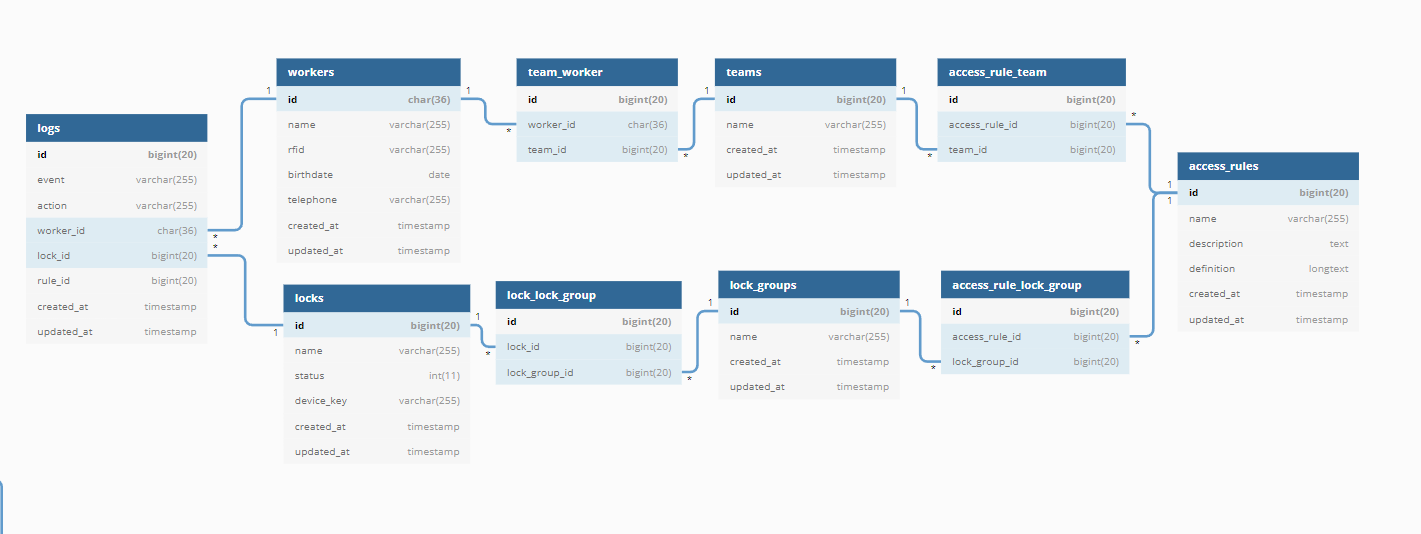
\includegraphics[width=1\textwidth]{images/model-connections.png}
            	\caption{Modellek kapcsolatai}
            	\label{fig-model-connections}
            \end{figure}
			
			\subsection{User}
				Azon fehasználók adatit tárolja, akik be tudnak jelentkezni az adminisztrációs felületre. A bejelentkeztetésért és jogosultságkezeléssel foglalkozó szolgáltatások ezzel a modellel dolgoznak. Alapbeállítás szerint egyedi UUID-t használ az adatbázis kulcsának, nem sorszámot, valamint a törlés alapértelmezett viselkedése \textqq{Soft-Delete}, tehát amikor egy felhasználót törlünk, akkor nem kerül ki az adatbázisból, csupán kitöltésre kerül egy \texttt{deleted\_at} mező. A Laravel ezt a legtöbb esetben úgy kezeli, hogy az ilyen rekordokat ignorálja, mintha törölve lennének, ugyan akkor bármikor könnyen visszaállíthatjuk ezeket. Így törlés helyett inkább csak deaktiválásról beszélünk.
				
			\subsection{Worker}
				Azon felhasználók adatait tárolja, akik a zárakat tudják használni. Egyedi UUID-t használ kulcsként, nem sorszámot. Álltalában tartozik hozzájuk valamilyen \textqq{ujjlenyomat} (\texttt{Fingerprint}), ami alapján azonosíthatóak. Ez lehet RFID kártya száma (ez a legvalószínűbb), felhasználónév, jelszó, de akár bináris adat is lehet. Ez utóbbi akkor szükséges, ha az azonosítást valamilyen komplex rendszer végzi, példáúl ujjlenyomat olvasó, de lehet akár retina szkenner is, stb.
				
			\subsection{Lock}
				A zárak adatait tárolja, amiket vezérelni szeretnénk. Itt ismételten található egy ujjlenyomat mező, ezúttal (az ütközések elkerülése végett) \texttt{device\_fingerprint} néven. Ez azért fontos, mert így felvihetjük például az eszközünk MAC címét, beégetett sorozatszámát, vagy bármilyen egyedi, nem módosítható adatot az eszközről, és a webservice ez alapján tudja azonosítani. A zár nem feltétlenül ajtó zárat jelent. Lehet akár egy szoftver is, ami függetlenül működik, és csak bejelentkezéshez használja ezt a rendszert.
				
				Minden zárhoz tartozik egy állapot. Ezek sorban:
				\begin{enumerate}
					\setcounter{enumi}{-1}
					\item Zárva (\emph{Locked}): Ez a zár nem enged át senkit.
					\item Müködésben (\emph{Operational}): Ez a zár csak azokat engedi át, akik valamilyen szabály szerint átmehetnek.
					\item Nyitva (\emph{Open}): Ez a zár mindenkit átenged, aki azonosítható, de a zár használatát naplózza.
					\item Ismeretlen (\emph{Unknown}): Ez a zár túl rég óta nem küldött életjelet (\emph{Keep-alive signal}), így a webservice nem tudja ellenőrizni az állapotát.
				\end{enumerate}
			
			\subsection{Group}
				Mind a Worker, mind pedig a Lock modell csoportokhoz rendelhető az egyszerűbb kezelhetőség érdekében. Köszönhetően a Laravel polimorfikus kapcsolatainak (\texttt{morphTo()} és \texttt{morphToMany()}) nem volt szükség külön-külön modellek létrehozására. A csoportok lényege, hogy amikor egy új zárat üzemelünk be, ne kelljen minden szabályt újra definiálnunk, ha már egyszer egy másik zár esetén megtettük.
				
			\subsection{Bouncer táblák}
				A Bouncer csomag négy modellt és az azokhoz tartozó adatbázis táblákat hozza létre nekünk. Ezek nagymértékben támaszkodnak a már említett polimorfikus kapcsolatokra, így bármilyen jogosultságot (\texttt{ability}-t) hozzá rendelhetünk bármilyen entitáshoz, illetve ezt a jogosultságot adhatjuk akár egy felhasználónak, akár egy jogkörnek (\texttt{role}).
			
		\section{AccessRule}
			A hozzáférési szabályok mondják meg a programnak, hogy átengedhet-e egy dolgozót egy záron. A szabály \textqq{egyik oldalán} (\texttt{operator}) állhat akár egy vagy több dolgozó, akár egy dolgozó csoport, tehát például nem muszáj két dolgozó miatt egy teljesen új csoportot létrehozni. 
			
			A szabály \textqq{másik oldalán} (\texttt{subject}) pedig állhat egy vagy több zár, vagy egy zár csoport is, tehát itt is érvényes az, hogy két zár miatt nem feltétlenül kell új csoportot létrehozni.
			
			A szabály definíciója JSON formátumban tárolódik. Maga a szabály lehet megengedő, vagy tiltó is. Továbbá definiálhatunk egy számlálót is, ami azt adja, hogy hányszor alkalmazható még ez a szabály. Ennél a számlálónál a \texttt{0} érték azt jelenti, hogy a szabály deaktiválva van, még a \texttt{-1}, vagy ha nincs jelen, az azt jelenti, hogy bármennyiszer alkalmazható.
			
			A szabályoknak két alakja van:
			\begin{enumerate}
				\item Speciális (\texttt{Specific})
				\item Általános (\texttt{Generic})
			\end{enumerate}
		
			\subsection{Speciális hozzáférési szabály}
				Ez egy olyan szabály, amit egy kifejezett idő intervallumra szeretnénk alkalmazni. Miután az intervallum lejárt a szabály törlődik.
				
				\begin{lstlisting}[caption={Egy p\'elda speci\'alis szab\'aly l\'etrehoz\'asa},captionpos=b][language=json]
{
  "operator_id": "5f1a20f7-368a-453e-b7ad-79b495b086b0",
  "operator_type": "Worker",
  "subject_id": "c15ad3b5-9e69-4eb7-9a8b-4bd76316d924",
  "subject_type": "Group",
  "count": 1,
  "definition": {
                 "from": "2021-06-04 10:00:00",
                 "to": "2021-06-04 18:00:00",
                 "allow": true
                }
}
				\end{lstlisting}
				
			\subsection{Általános hozzáférési szabály}
				Minden olyan szabály, ami nem idő intervallumhoz kötöt, vagy rendszeresen ismétlődik. Az \texttt{on\_every} tulajdonsággal definiálhatjuk, hogy mely napokon ismétlődik a szabály. Ezt a jelölést többféleképpen is megtehetjük. Felsorolhatjuk tömbben, hogy a hét hanyadik napjain érvényes a szabály, vagy szövegesen is megadhatjuk. A szöveges megadás jelenleg a következő definíciókat támogatja:
				\begin{itemize}
					\item \texttt{*}: Minden nap
					\item \texttt{weekday}: Minden hétköznap
					\item \texttt{weekend}: Minden hétvégén
				\end{itemize}
				Hogy a hét mely napjait számolja hétköznapnak és hétvégének, az személyre szabható. A \texttt{from} és \texttt{to} mező ekkor opcionális, alap értéke az adott napon \texttt{00:00:00.001} és \texttt{23:59:59.999}.
				
				\begin{lstlisting}[caption={Egy p\'elda \'altal\'anos szab\'aly l\'etrehoz\'asa},captionpos=b][language=json][firstnumber=1]
{
  "operator_id": "5f1a20f7-368a-453e-b7ad-79b495b086b0",
  "operator_type": "Worker",
  "subject_id": "c15ad3b5-9e69-4eb7-9a8b-4bd76316d924",
  "subject_type": "Group",
  "count": 1,
  "definition": {
                  "on_every": "*"
                  "from": "2021-06-04 10:00:00",
                  "allow": true
                }
}
			\end{lstlisting}
		
			Amennyiben a zár nyitási kérelmük mellé egyéb dolgozóval kapcsolatos adatot is csatolunk, úgy ezeket is ellenőrzi a rendszer. Ez például akkor hasznos, ha email cím - jelszó páros véd valamilyen zárat.
		
	\chapter{Admin Service}
		A beléptetőrendszer menedzselését célszerű egy admin felületen megtenni. Az alkalmazás alapból nem rendelkezik semmilyen felülettel, csak az API-on keresztül kommunikálhatunk vele. A szakdolgozatban mellékeltem egy Angular alapú Adminisztrátori felületet, mely teljesen függetlenül, SPA formában működik. Itt azonban kiemelném, hogy a szakdolgozat témája a webservice, és csupán demonstrációs céllal készült hozzá frontend, éppen ezért ezt a részt csak felületesen érintem.
		
		Az Admin Service futhat ugyanazon a szerveren, ahol a webservice, vagy teljesen különbözőn. Utóbbi esetben a \verb|FRONTEND_URL| és a \verb|FRONTEND_PORT| környezeti változók beállítása fontos, ugyanis ezek nélkül a web service CORS beaállítása letiltja az üzenet váltást.
		
		Egy valós szituációban az alkalmazó vállalkozás valószínüleg saját felületet írna erre a célra, így a dolgozat ezen részével csak felületesen foglalkozom.
		
		\section{Angular}
    		A forontend réteghez számtalan különböző technológia áll rendelkezésünkre, és ezek alatt nem csak a JavaScript keretrendszereket kell érteni, hiszen a projekt frontendje nem csak böngészőben futhat. Mivel a webservice csupán egy API-t biztosít, így csak az alkalmazón múlik, hogy milyen frontend-et ír hozzá.
    		
    		A demonstrációhoz én egy Angular-Ionic SPA (\verb|Single Page Application|) mellett döntöttem.
    		
    		Az Angular (nem összekverendő az AngularJS-el) egy nyílt forráskódú keretrendszer webes alkalmazásokhoz, amit arra terveztek, hogy az egyfejlesztős projektektől, akár a nagy céges szintű alkalmazásokig bármekkora projekt elkészíthető legyen úgy, hogy a kód tiszta, és egyszerűen karbantartható legyen. Az Angular teljes mértékben TypeScript-ben íródott, ami fantasztikus segédeszközök, és statikus típusok használatát teszi lehetővé. Továbbá legnagyobb pozitív tulajdonsága, hogy hatalmas mennyiségű könyvtár áll rendelkezésünkre, hogy megkönnyítse a fejlesztést.\cite{angular-intro}
    		
    		Az alkalmazás legalapvetőbb építőkövei a komponensek. Egy komponens lehet bármi, ami a felhasználónak megjelenik, például egy Beviteli mező, de a teljes oldal, amit megjelenítünk is csak egy komponens, ami más komponenseket ágyaz be. A kódban ezen komponenseket egy TypeScript osztály reprezentál, amit ellátunk az \verb|@Component()| dekorátorral. Ebbe az osztályba felvihetjük a funkcionalitáshoz szükséges kódot (Eseményeket, adatokat, stb.). A komponensekhez tartozik még egy \emph{Template} is, ami lényegében HTML kibővítve, illetve egy \emph{Style}, ami pedig SCSS, de az itt definiált stílusok csak az adott komponensben érvényesek.\cite{angular-components}
    		
    		Ezek a komponensek modulokba rendeződnek, amik egy fa architektúrában kapcsolódnak egymáshoz. Minden komponens csak a saját, és a \textqq{gyermek} modulokban elérhető.
    		
    		Az Angular ezek mellett biztosít nekünk egy automatikus \verb|Dependency Injector|-t is, ami leveszi az osztályok konstruálásának terhét rólunk. Amikor egy osztálynak szüksége van egy másikra, ahelyett, hogy létre kellene hoznunk azt (potenciálisan újabb föggőségeket létrehozva), elegendő az adott osztály konstruktorában megadni, hogy mire van szükségünk. Az Angular ezeket automatikusan feloldja. Ezek a injektálható osztályok automatikusan \emph{Singleton}-ként viselkednek, anélkül, hogy nekünk implementálni kellene a tervezési mintát.\cite{angular-di}
		
		\section{Ionic}\label{sc-ionic}
    		Az Ionic alapvetően egy eszközkészlet cross-platform alkalmazások fejlesztéséhez. Többek közt biztosít egy Angular csomagot, amiben számtalan javítás és kiegészítés van\cite{ionic-intro}. A három legfontosabb számomra az \emph{Ionic Router} (új \emph{life-cycle} metódusok), a \emph{Storage Service} (intelligens lokális tárhely kezelés), és az \emph{IonicServiceWorker} (PWA integráció).
    		
    		Az \emph{IonicServiceWorker} miatt, a felület \emph{PWA} (\emph{Progressive Web Application}) ként is működik. Az Ionic \emph{Capacitor} integrációt is biztosít. Ez azt jelenti, hogy szükség esetén a Frontend natív Android vagy IOS alkalmazás ként is lefordítható.\cite{ionic-cap}
    		
		\section{Felület}
		    Mivel a témám csupán a webservice, így nem szerettem volna túl sok időt a design részre fordítani, ugyan akkor azt sem szerrettem volna, hogy egy \textqq{fehér alapon fekete betűs} felületet adjak át mint szakdolgozat. Szerencsére, számtalan ingyenes és szabadon felhasználható előre kész felület érhető el Angular-ra is. Az én választásom a \emph{CoreUI}-ra esett. Az ez alapján készített nyító oldalt látni a \ref{fig-coreui-dash} ábrán.
		    
		    \begin{figure}[ht]
            	\centering
            	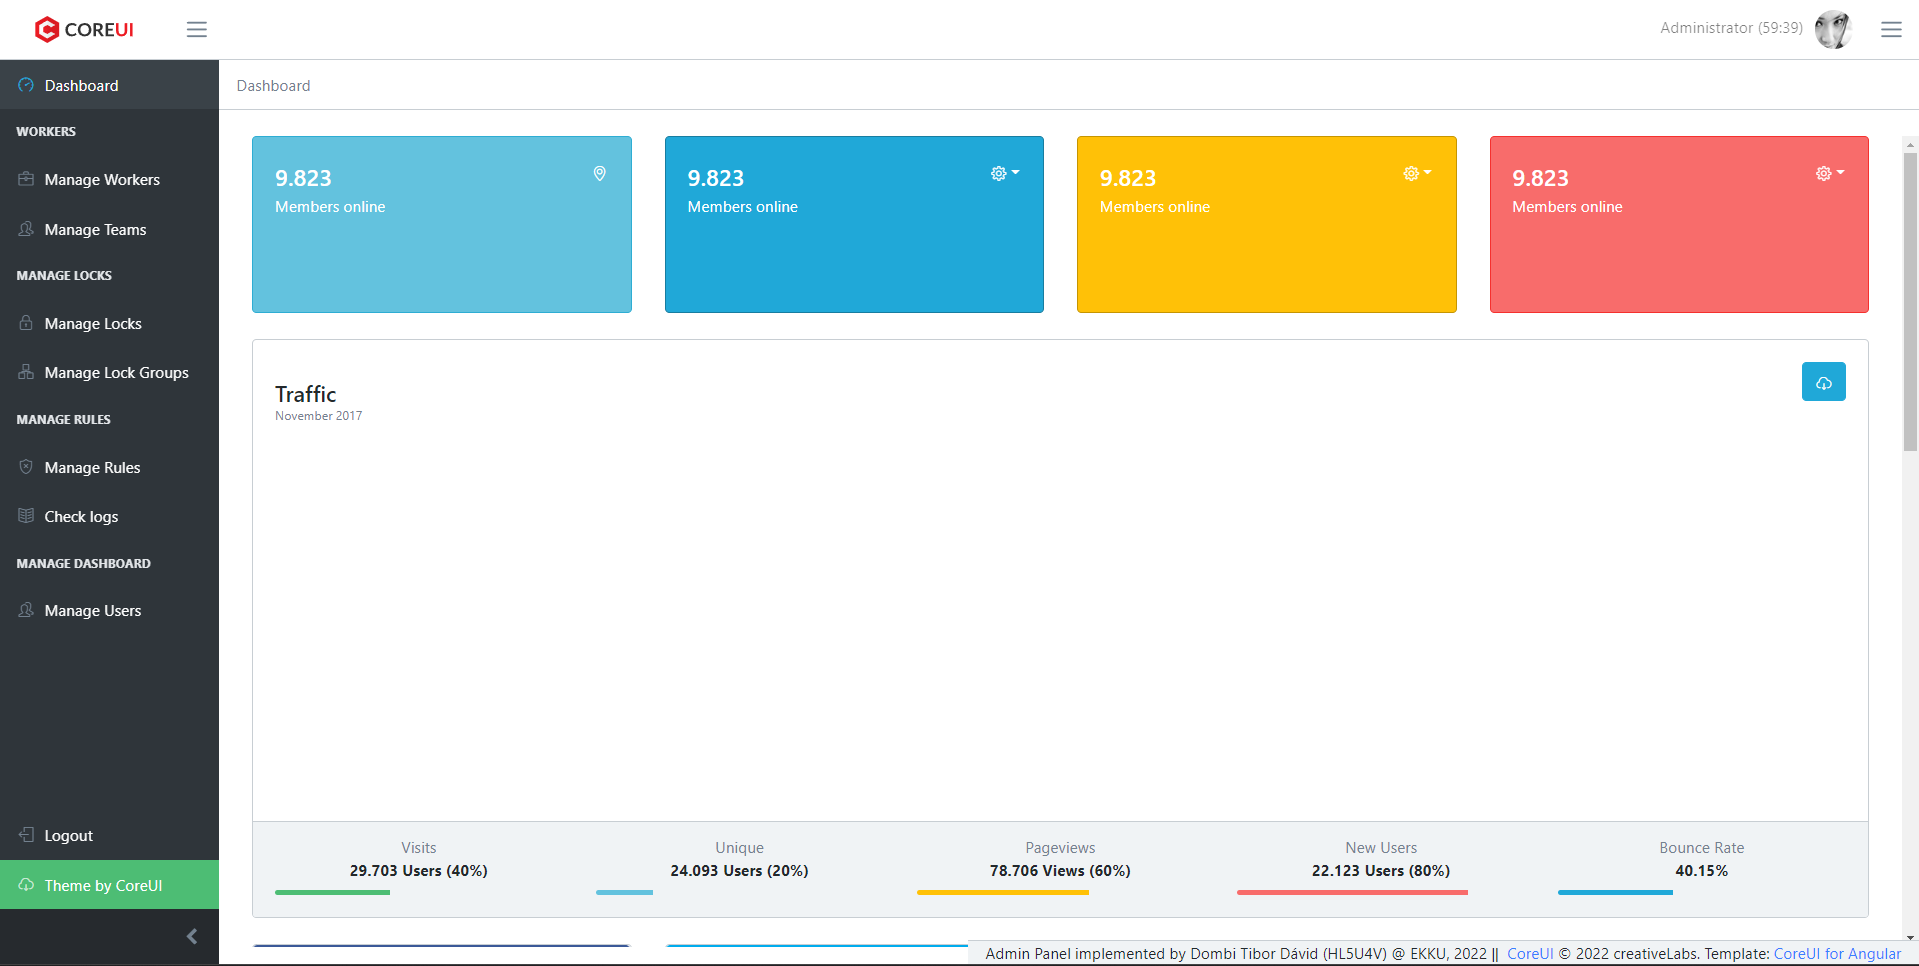
\includegraphics[width=1\textwidth]{images/coreui-dash.png}
            	\caption{Az admin fel\"ulet}
            	\label{fig-coreui-dash}
            \end{figure}
		    
		    Ez a csomag előre elkészített stíluslapokkal, komponensekkel, \emph{layout}-al érkezik, és gyakorlatilag nulla konfigurációra van szükség a használatához\cite{coreui-intro}. A csomag alapból Bootstrap4-et tartalmaz, ezt én Bootstrap5-re cseréltem. A csere után azonban a csomagok telepítése \emph{NPM}-el lehetetlenné vált kompatibilitási okokból, ugyanakkor \emph{Yarn}-al továbbra is probléma (és figyelmeztetések) nélkül működik. A szakdolgozat leadásáig ezt a hibát nem sikerült orvosolni, de mivel saját munkafolyamatomban Yarn-t használok ahol csak lehet, illetve azzal a telepítés probléma nélkül lefut, így nem is kezelem prioritásként.
		    
		    A CoreUI csomagot \emph{Łukasz Holeczek} készítette, és az MIT licensz alatt tette elérhetővé. Ez a projekt szintén MIT licenszt használ, és nem kerül eladásra semmilyen formában. Az eredeti licenszet én is mellékeltem a forráskódban az \verb|admin-panel| mappában\cite{coreui-mit}. Továbbá a felületen megtartottam a sablon weboldalára mutató linket (\ref{fig-coreui-dash} ábra, oldalsáv utolsó eleme).
		    
		    
		    \subsection{Adattábla komponens}
		    Mivel az összes erőforrásra, csak egyszerű CRUD műveleteket kell végeznünk, így nem érdemes mindet külön-külön implementálni. Sokkal célravezetőbb, ha készítünk egy univerzális komponenst, amit újra és újra fel tudunk használni az összes erőforráshoz. 
		    
		    Az admin panelben ez a \verb|CrudTableComponent|\footnote{Forráskód: \url{https://github.com/dombidav/hl5u4v-thesis/blob/main/admin-panel/src/app/shared-components/crud-table/crud-table.component.ts}}. Így elég csupán ezt elhelyezni a \emph{template}-ben, és megadni a megfelelő paramétereket. Ezek közül csak az \emph{erőforrás neve}, a \emph{megjelenítendő oszlopok}, illetve az erőforráshpz tartozó \emph{service} megadása kötelező. Opcionálisan letilthatjuk, vagy beállíthatjuk, hogy a keresés mely mezőkben történjen, figyelhetünk a különböző CRUD eseményekre, és még a táblázatuk stílusát is beállíthatjuk csupán a komponens paramétereivel. 
		    
		    \pagebreak
		    
		    A  \ref{cd-workers-template} kód a legegyszerűbb implementálást mutatja, kiegészítve a \verb|refreshTable| paraméterrel, ami egy \texttt{BehaviorSubject} (\texttt{speciális Observable}) példány. A változásán keresztül bármikor frissíthetjük a táblánkat a szülő komponensből. Erre azért van szükség, mert az \verb|<app-crud-table>| komponens nem tud arról, hogy megváltozott az adat, ha ezt a változtatást egy másik komponens teszi meg. Ilyen eset amikor a szerkesztéshez átnavigáljuk a felhasználót egy másik oldalra, majd vissza ide.
		    
		    	\begin{lstlisting}[caption={\texttt{workers.component.html}},captionpos=b,language=xml,label=cd-workers-template]
<app-layout>
    <app-crud-table 
    resourceName='Workers' 
        [refresh]='refreshTable' 
        [service]='workersService' 
        [columns]="columns">
    </app-crud-table>
</app-layout>
			\end{lstlisting}
			
			Ez az egyszerű kód (\ref{cd-workers-template}) a \ref{fig-coreui-workers} ábrán látható eredmény generálja nekünk. A táblázat oszlopai rendezhető növekvő vagy csökkenő sorrendben, szerkeszthetünk, létrehozhatunk és szerkeszthetjük az adatokat, illetve a kijelölés segítségével csoportosan is törölhetjük azokat. Mivel a komponens paraméterei között nem korlátoztuk a keresést, így az összes \emph{megjelenített} mezőben keres.
			
			\begin{figure}[ht]
            	\centering
            	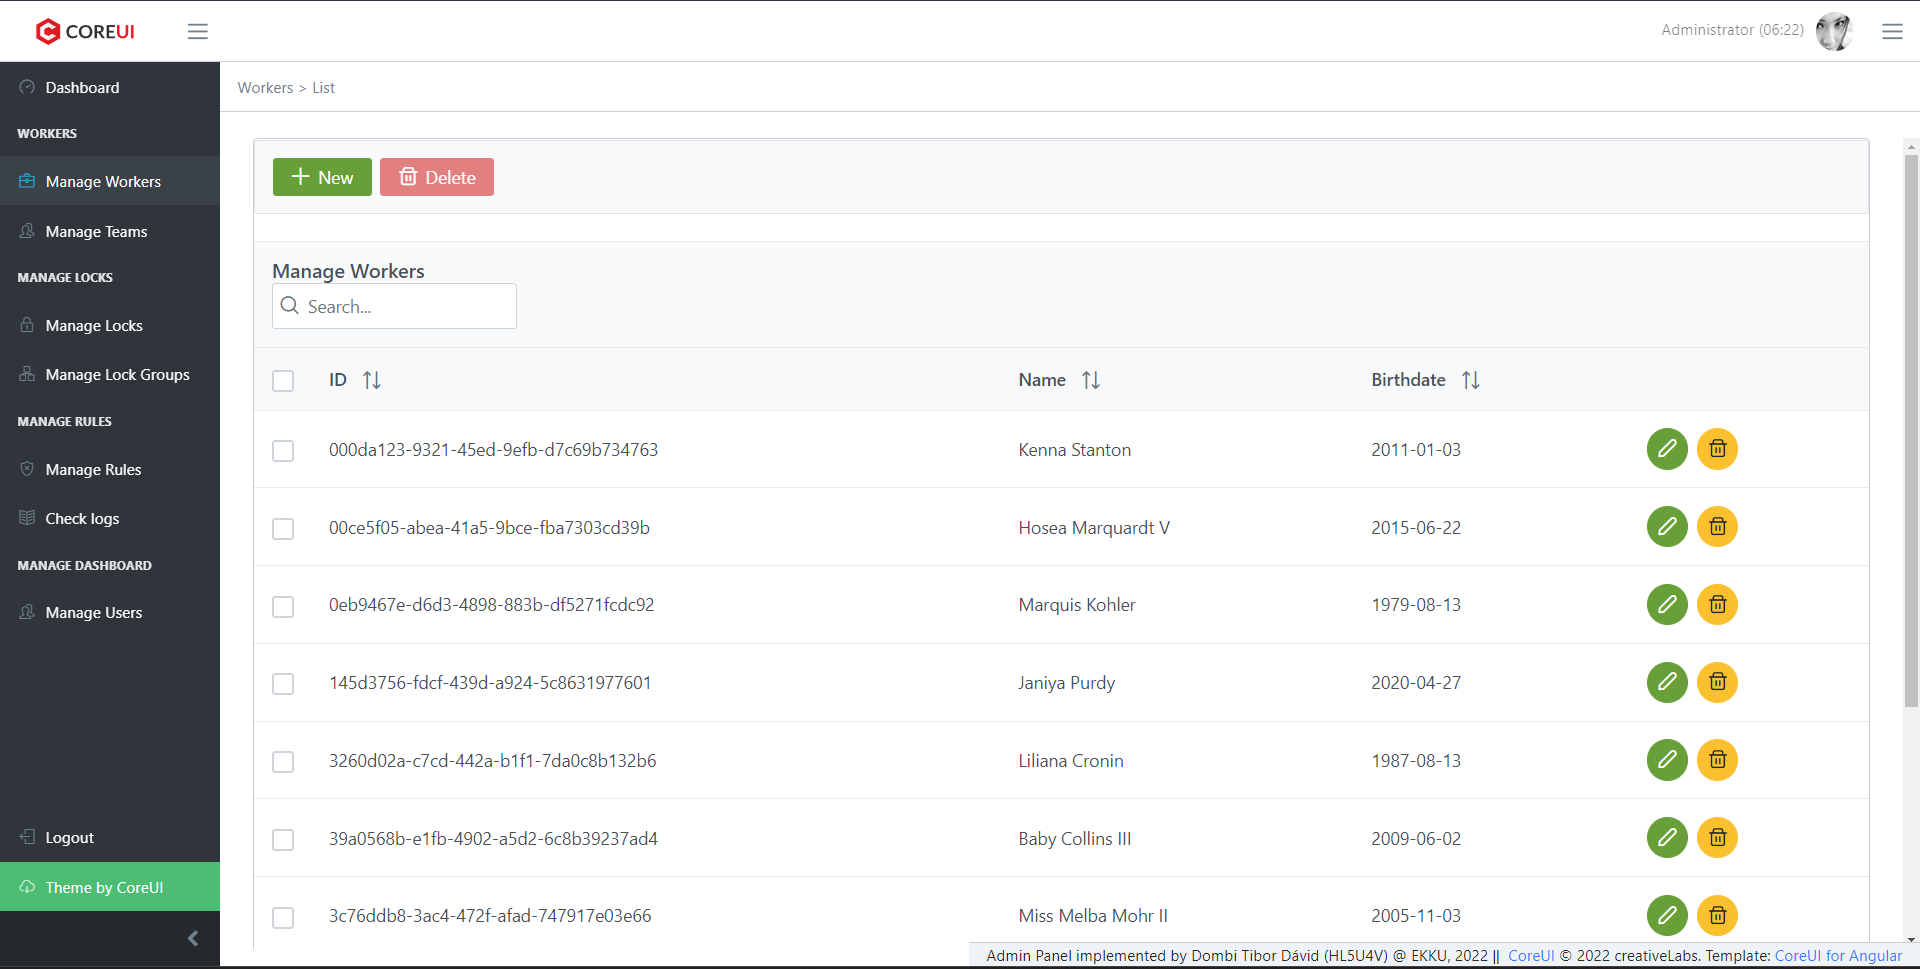
\includegraphics[width=1\textwidth]{images/coreui-workers.png}
            	\caption{A \texttt{CrudTableComponent} megjelenése}
            	\label{fig-coreui-workers}
            \end{figure}
		    
    		
		
    		
	\chapter{Hardveres megvalósítási javaslat}\label{ch-Hardware}
		Bár a szakdolgozat csak a webservice résszel foglalkozik, mint projekt úgy gondolom fontos javaslatot tenni a hardveres megvalósításra, ha más miatt nem is, legalább azért hogy egy alapot adjon annak, aki ténylegesen szeretné beüzemelni az alkalmazást. Természetesen számtalan módon megoldható az eszközök összekapcsolása, valamint a webservice-al való kommunikáció, ez amit ide írok egy példa csupán.
		
		\section{Elosztott rendszerű megoldás}
			Ebben a példa szituációban minden zárt valamilyen Wi-Fi képes mikrokontroller vezérel. Az \texttt{ESP8266} egy viszonylag olcsó ilyen eszköz. Kössük hozzá a zármechanika motorját, illetve a leolvasónkat, ami legyen példáúl egy RFID leolvasó. Ezután az ESP-nkkel kapcsolódjunk Wi-Fi-n keresztül az internetre. Az ESP rendelkezik egy beégetett gyártási számmal (\texttt{Device ID}), ez lesz az eszközünk ujjlenyomata (Például: \texttt{f84020329c0e}).
			
			Amikor egy dolgozó a leolvasóhoz érinti a saját RFID kártyáját, akkor az ESP a kártya azonosítóját olvassa, és nem a dolgozóét, ezért az adatfelvitelkor a kártya azonosítóját kell megadjuk mint a dolgozó ujjlenyomata (példáúl: \texttt{f3949935-5425-4879-b713-bd9f3bd77241}). A leolvasás után az ESP HTTP POST kérést indít a webservice felé, ami így néz ki (API-KEY hitelesítéssel):
			
			\begin{lstlisting}[caption={Elosztott rendszer HTTP k\'er\'ese},captionpos=b]
POST /api/acs/confirm/f84020329c0e
Host: www.acs.example.com
Content-Type: application/json; charset=utf-8
Content-Length: {LENGTH}
Accept: application/json
X-API-KEY: kLhIlqOvCRcawFlD-tdMBPCHDUGhtuCuO

{
	"worker_rfid": "f3949935-5425-4879-b713-bd9f3bd77241"
}
			\end{lstlisting}
			
			Figyeljük meg, hogy az eszköz ujjlenyomata az URI-ben kapott helyet. Ezt az ujjlenyomatot nyugodtan kicserélhetjük az eszköz tényleges, adatbázisban használt kulcsára, a hitelesítés akkor is működni fog. Ezután a szerver vagy engedélyezi, vagy valamilyen hiba üzenettel válaszol.
			
		\section{Csillagpontos megoldás}
			Amennyiben nem szeretnénk minden zárhoz külön-külön mikrokontrollert elhelyezni, elképzelhető az is, hogy egy nagyobb, több csatolakozási lehetőséggel rendelkező vezérlő egységet használunk (például egy Raspberry Pi-t), és ehhez, csillagpontosan hozzákötünk minden zárat és minden leolvasót. 
			
			A leolvasásra hasonlóan reagál, mint az elosztott rendszer, de itt a vezérlőnek tudnia kell, hogy melyik leolvasó melyik zárhoz tartozik. Az üzenet URI-jében az adott zár ujjlenyomatát kell használni. Arra nincs szükség, hogy a vezérlő az API kulcsát is ismerje minden egyes zárnak, használhatja minden lekéréshez a saját API kulcsát. 
			
	\chapter{Továbbfejlesztési lehetőségek}\label{ch-todo}
		Természetesen, mint minden szoftver, ez az alkalmazás is rendelkezik hibákkal, hiányosságokkal. Ezeket a jövőben érdemes lenne kijavítani, vagy néhol újra gondolni.
		
		\section*{Bejelentkezés és Regisztráció}
			A bejelentkezés és a regisztráció során a felhasználó adatai (kiemelten a jelszó) titkosítatlanul kerülnek átadásra, és csak a szerveren kezeltem le. Ezt jó lenne már a kliens oldalon titkossá tenni. Erre megoldást jelenthet a JWT.
			
		\section*{Képek feltöltése}
			Jelenleg a webservice nem támogatja a képek feltöltését, pedig mind az adminisztrátori felület használóit, mind a dolgozókat könnyebb lenne beazonosítani.
		
		\section*{Modellek}
			Fentebb már részleteztem az Eloquent problémáit (lásd: \ref{sc:eloquent} - \nameref{sc:eloquent} fejezet), ezt orvosolandó implementálni lehetne a \texttt{repository pattern} irányelveit.
		
		\section*{Rest API helyett GraphQL}
			Az alkalmazás méreteiből adódóan messze túl sok végponttal rendelkezik. Ez orvosolható lenne azzal, ha hagyományos Restful API helyett GraphQL-t használna az alkalmazás.
		
		\section*{Adminisztrátori tevékenységek naplózása}
			Jelenleg csak a zárak használata, valamint a Laravel-el kapcsolatos események kerülnek naplózásra. Érdemes lenne az olyan eseményeket is feljegyezi, mint példáúl, ha valaki új rekordot vitt fel, vagy épp törölt egyet.
			
		\section*{Szabály definíció tisztázása}
			A mostani struktúrája a hozzáférési szabály definícióknak elég körülményes, és nem evidens. Érdemes lenne új struktúrában gondolkodni.
			
		\section*{Bouncer csomag elvetése}
			Bár szintaxisa miatt igen kedvelt csomag, sajnos mind teljesítményben, mind korlátoltsága miatt alulmarad a \texttt{Laravel Spatie}-vel szemben. 
			
		\section*{MongoDB támogatás}
			Habár sem a Laravel, sem a PHP nem támogatja alapból a MongoDB adatbázisokat, a PHP a megfelelő kiegészítővel, a Laravel pedig a megfelelő csomag telepítésével, viszonylag egyszerűen képessé tehető rá. A MongoDB egyre nagyobb népszerűségnek örvend az elmúlt években, így egyáltalán nem elképzelhetetlen, hogy valaki ezt szeretné használni az alkalmazáshoz. Azonban ekkor két probléma merül fel:
			
			Az első, hogy a Bouncer egészen egyszerűen nem képes a Mongo környezetben működni.
			
			A második, hogy a \texttt{MongoDB-Eloquent} csomag használatához egy teljesen másik absztrakt Model osztálytól kell örököltetnünk a modelljeinket, és a két absztrakt osztálynak nincs közös őse, így nem lehet egyszerűen \textqq{kicserélni} egyiket a másikkal. A legtöbb beépített függvény a Laravelben pedig az eredeti Model típust várja paramétereiben.
			
	\chapter*{Összegzés}
    	A projekt célja az volt, hogy egy könnyen integrálható és tovább fejleszthető beléptetőrendszer szoftveres megoldása legyen. Rendkívül fontos volt számomra, hogy minél inkább nyitottá tegyem a projektet a közösség számára, méghozzá úgy, hogy ne csak egyszerűen elérhetővé tegyem a forráskódot, de minél több eszközt és dokumentációt mellékeljek.
    	Továbbá, az alkalmazás természetesen nyitott a közösségi fejlesztés felé is.
    	
    	A szakdolgozat leadása után a projekt fejlesztése nem áll meg. Mindenképpen implementálni szeretném a továbbfejlesztési lehetőségek között leírtakat, felhasználóbarátabbá tenni az admin felületet, illetve valós, fizikai megvalósítás is tervben van. Remélem, hogy ezt már a közösséggel együtt tehetem majd meg.
    	
    	A rendszer második verzióját úgy tervezem megvalósítani, hogy programozói tudás nélkül is beüzemelhető és használható legyen. Ez a verzió akár szolgáltatásként is nyújtható lesz, folyamatos támogatás mellett. Tanulmányaimat követően elképzelhetőnek tartom, hogy majd saját vállalkozásomban foglalkozom ezzel a tovább fejlesztett verzióval.
    	
    	Úgy gondolom, hogy hiányosságai ellenére a projekt jelen állapotában is alkalmazható egy valós probléma megoldására.
	
	\chapter*{Köszönetnyilvánítás}
    	Szeretnék köszönetet mondani egyetemi oktatóimnak a tőlük kapott tudásért és segítségért.
    	
    	Külön köszönöm Dr. Tajti Tibor segítségét ebben a projektben és egyéb dolgokban, valamint azért, hogy szakmai gyakorlatom alatt bevezetett az IoT világába.
    	
    	Köszönöm hallgatótársaimnak, barátaimnak, hogy mindig voltak köztük olyanok, akik segíteni tudtak és figyeltek rám.
    
    	Végül de nem utolsó sorban szeretnék köszönetet mondani szüleimnek, családomnak, hogy mellettem álltak, és tanulmányaim alatt végig támogattak.
			
\begin{thebibliography}{2}

    \bibitem{octoverse}Github Octoverse Statisztika 2021,
    \\\texttt{\url{https://octoverse.github.com/}}
    
    \bibitem{phpstatistics}PHP Market Share és statisztikák
    \\\texttt{\url{https://w3techs.com/technologies/details/pl-php}}
    
    \bibitem{repo}Projekt GitHub repository-ja
    \\\texttt{\url{https://github.com/dombidav/hl5u4v-thesis}}
    
    \bibitem{php-servers}PHP Szerverek
    \\\texttt{\url{https://serverguy.com/servers/php-servers/}}
    
    \bibitem{supported-dbms}Laravel által támogatott DBMS-ek
    \\\texttt{\url{https://laravel.com/docs/9.x/database}}
    
    \bibitem{sail-intro}Laravel Sail
    \\\texttt{\url{https://laravel.com/docs/9.x/sail}}
    
    \bibitem{install-wizard-js}Telepítő varázsló forráskódja
    \\\texttt{\url{https://github.com/dombidav/hl5u4v-thesis/blob/main/scripts/install-wizard.js}}
    
    \bibitem{postinstall}Postinstall dokumentáció
    \\\texttt{\url{https://yarnpkg.com/package/postinstall}}
    
    \bibitem{yarn}Yarn
    \\\texttt{\url{https://classic.yarnpkg.com/en/docs/cli/install}}
    
    \bibitem{redis-as-cache}Redis mint Cache
    \\\texttt{\url{https://www.honeybadger.io/blog/laravel-caching-redis}}
    
    \bibitem{laravel-mail}Laravel Mail
    \\\texttt{\url{https://laravel.com/docs/9.x/mail}}
    
    \bibitem{gh-actions}Github Actions
    \\\texttt{\url{https://github.com/features/actions}}
    
    \bibitem{heroku}Heroku
    \\\texttt{\url{https://devcenter.heroku.com/articles/how-heroku-works}}
    
    \bibitem{phpunit}PHP Unit
    \\\texttt{\url{https://phpunit.readthedocs.io/en/9.5/writing-tests-for-phpunit.html}}
    
    \bibitem{artisan-test}Artisan Teszt a Laravel dokumentációjában
    \\\texttt{\url{https://laravel.com/docs/9.x/console-tests\#input-output-expectations}}
    
    \bibitem{ci-cd}Mi a CI/CD, bevezető
    \\\texttt{\url{https://www.redhat.com/en/topics/devops/what-is-ci-cd}}
    
    \bibitem{rest-api}Mi a RestAPI
    \\\texttt{\url{https://www.redhat.com/en/topics/api/what-is-a-rest-api}}
    
    \bibitem{open-api}OpenAPI definíció
    \\\texttt{\url{https://github.com/dombidav/hl5u4v-thesis/blob/main/docs/openapi.json}}
    
    
    \bibitem{stoplight}OpenAPI definíció a stoplight.io-n
    \\\texttt{\url{https://hl5u4v-thesis.stoplight.io/docs/hl5u4v-thesis/branches/main/}}
    
    \bibitem{bread}Bread vs. CRUD
    \\\texttt{\url{https://www.reddit.com/r/webdev/comments/3l2vio/buttonaction_language_crud_vs_bread/}}
    
    \bibitem{http}HTTP metódusok
    \\\texttt{\url{https://www.restapitutorial.com/lessons/httpmethods.html}}
    
    \bibitem{uri}URI, erőforrás azonosítás
    \\\texttt{\url{https://developer.mozilla.org/en-US/docs/Web/HTTP/Basics_of_HTTP/Identifying_resources_on_the_Web}}
    
    \bibitem{sanctum}Laravel Sanctum és a policy-k használata együtt
    \\\texttt{\url{https://laracasts.com/discuss/channels/laravel/how-to-use-policies-with-laravel-sanctum}}
    
    \bibitem{jwt-intro}JWT bevezető
    \\\texttt{\url{https://jwt.io/introduction}}
    
    \bibitem{jwt-handbook}JWT Handbook
    \\\texttt{Sebastián E. Peyrott, Auth0 Inc (Version 0.14.1, 2016-2018)}
    \\\texttt{\url{https://assets.ctfassets.net/2ntc334xpx65/o5J4X472PQUI4ai6cAcqg/13a2611de03b2c8edbd09c3ca14ae86b/jwt-handbook-v0_14_1.pdf}}
    
    \bibitem{jwt-workflow}JWT Usecase Workflow
    \\\texttt{\url{https://documentation.softwareag.com/webmethods/api_gateway/yai10-5/10-5_API_Gateway_webhelp/index.html\#page/api-gateway-integrated-webhelp/co-jwt_usecase_workflow.html}}
    
    \bibitem{laravel-wiki}Laravel, Wikpedia the free Encyclopedia
    \\\texttt{\url{https://en.wikipedia.org/wiki/Laravel}}
    
    \bibitem{framework-comp}Devecosystem 2020, PHP
    \\\texttt{\url{https://www.jetbrains.com/lp/devecosystem-2020/php/}}
     
    \bibitem{laravel-eloquent}Eloquent, Laravel Docs
    \\\texttt{\url{https://laravel.com/docs/9.x/eloquent}}
    
    \bibitem{eloquent-critics}The biggest problem with eloquent accessors magic
    \\\texttt{\url{https://laraveldaily.com/the-biggest-problem-with-eloquent-accessors-magic/}}
    
    \bibitem{database-testing}Database testing, Laravel Docs
    \\\texttt{\url{https://laravel.com/docs/9.x/database-testing/}}
    
    \bibitem{repository-pattern}Repository Pattern in Laravel Application
    \\\texttt{\url{https://www.twilio.com/blog/repository-pattern-in-laravel-application}}
    
    \bibitem{migration-docs}Database: Migrations, Laravel Docs
    \\\texttt{\url{https://laravel.com/docs/9.x/migrations}}
    
    \bibitem{migration-sqlite}Migration probléma SQLite adatbázis alatt. 
    \\\texttt{(Megjegyzés: A szakdolgozati projekt létrehozásakor a probléma még fennált)}
    \\\texttt{\url{https://github.com/laravel/framework/issues/35162}}
    
    \bibitem{bouncer-gate}Bouncer, Authorizing Users
    \\\texttt{\url{https://github.com/JosephSilber/bouncer\#authorizing-users}}
    
    \bibitem{angular-intro}Angular.io, What is Angular?
    \\\texttt{\url{https://angular.io/guide/what-is-angular}}
    
    \bibitem{angular-components}Angular.io, Components
    \\\texttt{\url{https://angular.io/guide/what-is-angular\#components}}
    
    \bibitem{angular-di}Angular.io, Dependency Injection
    \\\texttt{\url{https://angular.io/guide/what-is-angular\#dependency-injection}}
    
    \bibitem{ionic-intro}Ionic Dokumentáció
    \\\texttt{\url{https://ionicframework.com/docs}}
    
    \bibitem{ionic-cap}Ionic Dokumentáció, Capacitor integráció
    \\\texttt{\url{https://ionicframework.com/docs/developing/android\#running-with-capacitor}}
    
    \bibitem{coreui-intro}CoreUI Dokumentáció
    \\\texttt{\url{https://coreui.io/angular/docs/4.0/getting-started/introduction}}
    
    \bibitem{coreui-mit}Mellékelt CoreUI Licensz
    \\\texttt{\url{https://github.com/dombidav/hl5u4v-thesis/blob/main/admin-panel/LICENSE}}
    
    \includepdf{nyilatkozat.pdf}
    
\end{thebibliography}
		
\end{document}